\documentclass[tikz,border=6pt]{standalone}
\usepackage{amsmath,amssymb}
\usetikzlibrary{positioning,arrows.meta,calc,decorations.pathreplacing}

% ------ palette (mirror _ct_palette.py blue_ramp(8): H1 darkest -> H8 lightest) ------
\definecolor{CT}{HTML}{1F5C8B}
\definecolor{NOTc}{HTML}{B4513C}
\definecolor{INKc}{HTML}{1A1A1A}
\definecolor{CINPUT}{HTML}{E9F2E9}
\definecolor{CEMBED}{HTML}{DDEBF7}
\definecolor{CATTN}{HTML}{FDF2E3}
\definecolor{CAGG}{HTML}{E3F0E4}
\definecolor{CDAG}{HTML}{FBE4DF}
\definecolor{COUT}{HTML}{EDE6F5}
\definecolor{CBORD}{HTML}{333333}
\definecolor{CARROW}{HTML}{4A4A4A}
\definecolor{HLOSS}{HTML}{FBF0DC}
\definecolor{HLOSSBD}{HTML}{C9A15A}
\definecolor{TXTSUB}{HTML}{555555}
\definecolor{TXTGRAY}{HTML}{8A5A00}
\definecolor{H1}{HTML}{1F5C8B}
\definecolor{H2}{HTML}{38709A}
\definecolor{H3}{HTML}{4F81AD}
\definecolor{H4}{HTML}{6B97B8}
\definecolor{H5}{HTML}{85ABC7}
\definecolor{H6}{HTML}{9EBED7}
\definecolor{H7}{HTML}{B8D2E6}
\definecolor{H8}{HTML}{D1E6F5}

\begin{document}
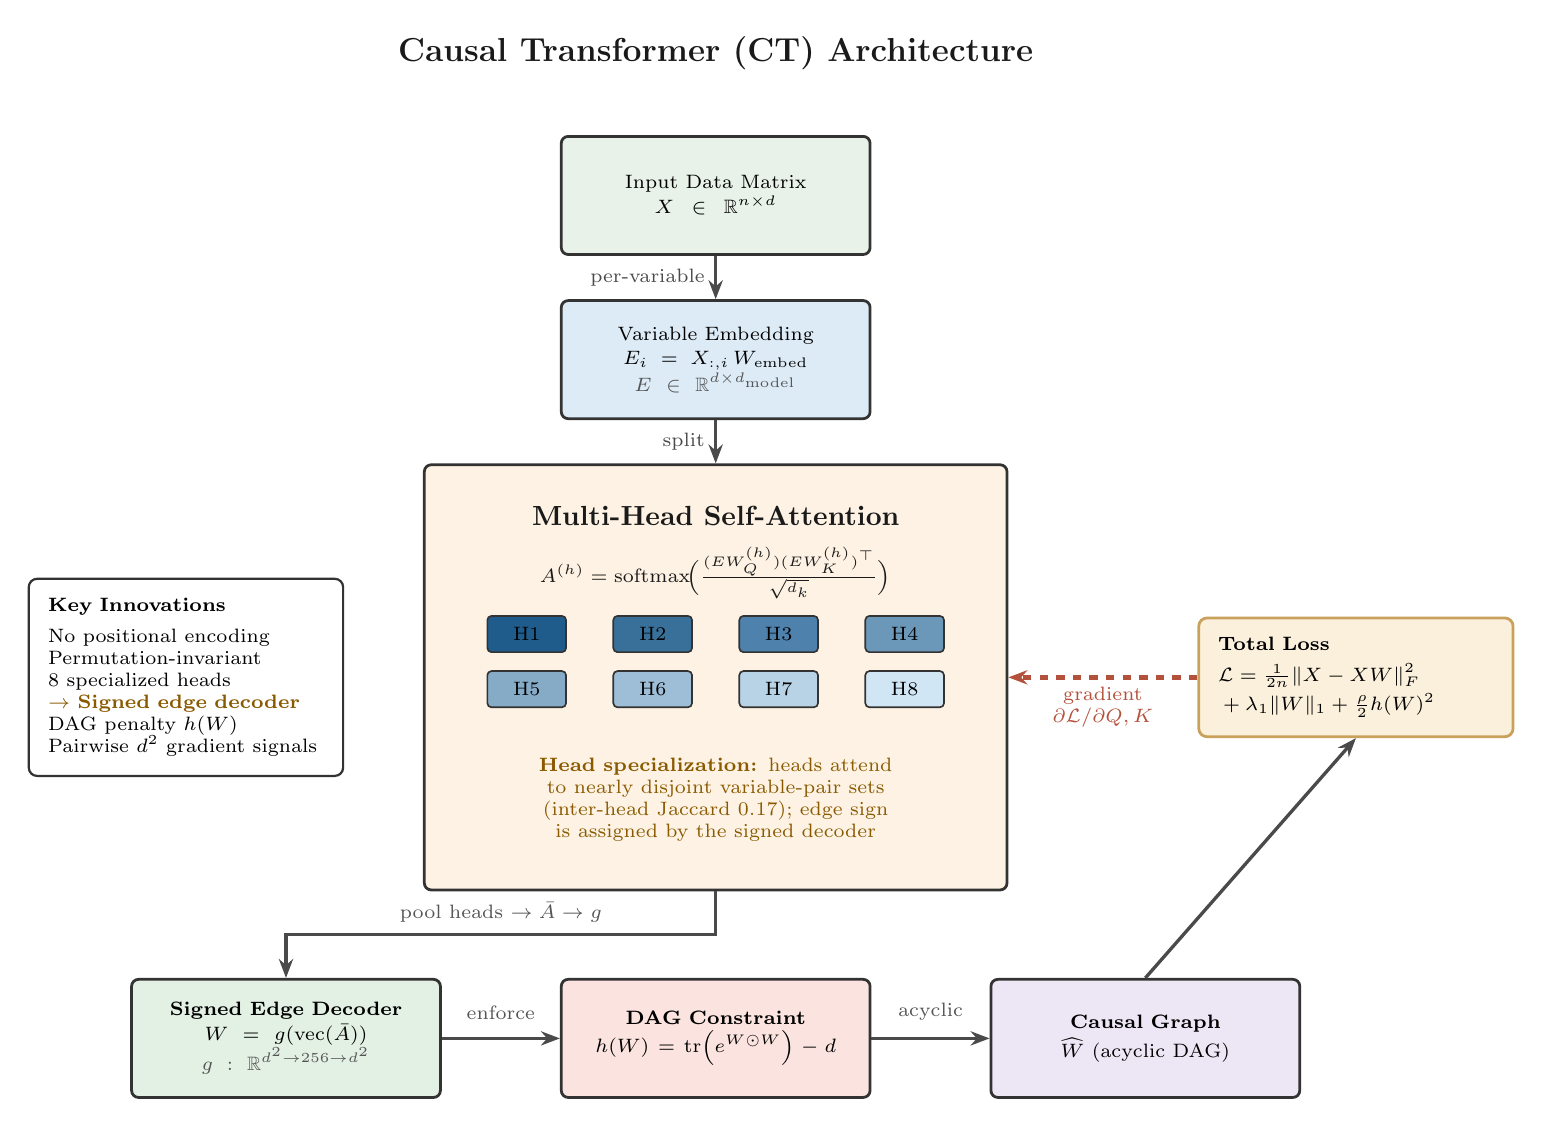
\begin{tikzpicture}[
  font=\scriptsize,
  % main content box: fixed text width so it never grows and collides with neighbours
  nbox/.style={draw=CBORD, line width=1.0, rounded corners=2.5pt, align=center,
               inner sep=6pt, text width=3.5cm, minimum height=1.5cm},
  % side panel box
  wbox/.style={draw=CBORD, line width=0.8, rounded corners=3pt, align=left,
               inner sep=7pt, text width=3.5cm, fill=white},
  % head chip
  head/.style={draw=CBORD, line width=0.6, rounded corners=1.5pt,
               minimum width=1.0cm, minimum height=0.46cm, align=center},
  % arrow style
  ar/.style={-{Stealth[length=2.4mm]}, color=CARROW, line width=1.2},
  % attention container
  bg/.style={draw=CBORD, line width=1.0, rounded corners=2.5pt,
             fill=CATTN, inner sep=0pt, minimum height=5.4cm, minimum width=7.4cm},
]

% ---------- Title ----------
\node[font=\large\bfseries, color=INKc] (TITLE) {Causal Transformer (CT) Architecture};

% ---------- Main stem (all relative positioning -> no overlap) ----------
\node[nbox, fill=CINPUT, below=0.7cm of TITLE] (IN)
  {Input Data Matrix\\[1pt]\scriptsize $X\in\mathbb{R}^{n\times d}$};
\node[nbox, fill=CEMBED, below=0.55cm of IN] (EM)
  {Variable Embedding\\[1pt]\scriptsize $E_i = X_{:,i}\,W_{\text{embed}}$\\
   \textcolor{TXTSUB}{\scriptsize $E\in\mathbb{R}^{d\times d_{\text{model}}}$}};
\draw[ar] (IN.south) -- node[left, pos=0.5]{per-variable} (EM.north);

% ---------- Attention container ----------
\node[bg, below=0.55cm of EM] (ATTN) {};
\node[font=\bfseries, color=INKc] (AN) at ($(ATTN.center)+(0,2.05)$) {Multi-Head Self-Attention};
\node[font=\scriptsize, color=INKc, align=center] (AE) at ($(ATTN.center)+(0,1.32)$)
  {$A^{(h)}=\mathrm{softmax}\!\Big(\frac{(EW_Q^{(h)})(EW_K^{(h)})^\top}{\sqrt{d_k}}\Big)$};
% 8 heads: 2 rows x 4 cols, centred inside container
\foreach \i/\xx/\hh in {1/-2.4/H1, 2/-0.8/H2, 3/0.8/H3, 4/2.4/H4}
  \node[head, fill=\hh] (h\i) at ($(ATTN.center)+(\xx,0.55)$) {H\i};
\foreach \i/\xx/\hh in {5/-2.4/H5, 6/-0.8/H6, 7/0.8/H7, 8/2.4/H8}
  \node[head, fill=\hh] (h\i) at ($(ATTN.center)+(\xx,-0.15)$) {H\i};
\node[text width=6.9cm, align=center, font=\scriptsize, color=TXTGRAY] (HN) at ($(ATTN.center)+(0,-1.55)$)
  {\textbf{Head specialization:} heads attend to nearly disjoint variable-pair sets\\
   (inter-head Jaccard $0.17$); edge sign is assigned by the signed decoder};
\draw[ar] (EM.south) -- node[left, pos=0.5]{split} (ATTN.north);

% ---------- Side panels (vertically centred on the attention container) ----------
\node[wbox, left=1.0cm of ATTN] (KI)
  {\textbf{Key Innovations}\\[3pt]
   \scriptsize No positional encoding\\ Permutation-invariant\\ 8 specialized heads\\
   \textcolor{TXTGRAY}{\bfseries $\to$ Signed edge decoder}\\ DAG penalty $h(W)$\\
   Pairwise $d^2$ gradient signals};
\node[wbox, draw=HLOSSBD, line width=1.0, fill=HLOSS, right=2.4cm of ATTN] (LOSS)
  {\textbf{Total Loss}\\[3pt]
   \scriptsize $\mathcal{L}=\frac{1}{2n}\|X-XW\|_F^2$\\[1pt]
   \scriptsize ${}+\lambda_1\|W\|_1+\frac{\rho}{2}h(W)^2$};

% ---------- Bottom row (DAG centred on x=0 so the row is balanced) ----------
\node[nbox, fill=CDAG, below=1.1cm of ATTN] (DAG)
  {\textbf{DAG Constraint}\\[1pt]\scriptsize $h(W)=\mathrm{tr}\!\left(e^{W\odot W}\right)-d$};
\node[nbox, fill=CAGG, left=1.5cm of DAG] (DEC)
  {\textbf{Signed Edge Decoder}\\[1pt]\scriptsize $W=g(\mathrm{vec}(\bar{A}))$\\
   \textcolor{TXTSUB}{\scriptsize $g:\mathbb{R}^{d^2\to256\to d^2}$}};
\node[nbox, fill=COUT, right=1.5cm of DAG] (OUT)
  {\textbf{Causal Graph}\\[1pt]\scriptsize $\widehat{W}$ (acyclic DAG)};

% ---------- Attention -> pool -> Decoder (jog above the row, clean) ----------
\draw[ar] (ATTN.south) -- ++(0,-0.55) coordinate (p) -- (p -| DEC.north) -- (DEC.north);
\node[font=\scriptsize, color=TXTSUB, anchor=south, yshift=0.03cm]
  at ($(p)!0.5!(p-|DEC.north)$) {pool heads $\to\bar{A}\to g$};

% ---------- DEC -> DAG -> OUT ----------
\draw[ar] (DEC.east) -- (DAG.west);
\node[font=\scriptsize, color=TXTSUB, anchor=south, yshift=0.11cm]
  at ($(DEC.east)!0.5!(DAG.west)$) {enforce};
\draw[ar] (DAG.east) -- (OUT.west);
\node[font=\scriptsize, color=TXTSUB, anchor=south, yshift=0.11cm]
  at ($(DAG.east)!0.5!(OUT.west)$) {acyclic};

% ---------- OUT -> Total Loss (output feeds the loss, thin grey) ----------
\draw[ar] (OUT.north) -- (LOSS.south);

% ---------- Total Loss -> Attention heads (dashed red back-prop gradient) ----------
\draw[-{Stealth[length=2.4mm]}, color=NOTc, line width=1.8, dashed]
  (LOSS.west) -- (ATTN.east);
\node[font=\scriptsize, color=NOTc, anchor=north, align=center]
  at ($(LOSS.west)!0.5!(ATTN.east)$) {gradient\\ $\partial\mathcal{L}/\partial Q,K$};

\end{tikzpicture}
\end{document}
